\documentclass{article}

% Language setting
% Replace `english' with e.g. `spanish' to change the document language
\usepackage[english]{babel}

% Set page size and margins
% Replace `letterpaper' with`a4paper' for UK/EU standard size
\usepackage[letterpaper,top=2cm,bottom=2cm,left=3cm,right=3cm,marginparwidth=1.75cm]{geometry}

% Useful packages
\usepackage{amsmath}
\usepackage{graphicx}
\usepackage[colorlinks=true, allcolors=blue]{hyperref}

\title{Machine Learning \\ Exercise 7: Manual calculation of the forward and backward pass for a simple Neural Network}
\author{Prof. Dr. Thomas Kopinski}

\begin{document}
\maketitle

\begin{abstract}
This exercise focuses on getting a deeper understanding of the inner workings of a simple neural network by making you perform the calculations and resulting weight updates by hand.
\end{abstract}

\section*{Task 1: Understand the algorithm}

\begin{itemize}
    \item Information about neural networks can be found in the materials accompanying this course as well as  \href{https://github.com/DataScienceLabFHSWF/machine-learning-book/blob/main/notebooks/ch09/ch09.ipynb}{here}.
    \item Make sure you understand how the data is propagated through the different layers of the neural network, especially during the backward pass.
    \item The calculations should be written down by hand and you should be able to explain the equations.
\end{itemize}

\section*{Task 2: Calculate the results of the forward pass}

\begin{itemize}
    \item The network plus its parameter values can be found in fig. \ref{fig:markers} on the next page. The Sigmoid function ($S(x) = \frac{1}{1+e^x}$) is used for activation of the network's neurons.
    \item Calculate the results of the forward pass for the two neurons in the hidden layer and additionally the output layer. The "target" values represent the expected/correct values for the input data.
\end{itemize}

\section*{Task 3: Calculate the results of the backward pass and update the network weights}

\begin{itemize}
    \item Use the results from Task 2 to determine the correct values for the updated weights.
    \item Make sure you write down the derivations that are needed in order to fulfill this exercise.
    \item Your task is to calculate the updated values for all weights after the first backward pass.
    \item The \emph{learning rate} for this network is set to 0.1.
    \item Tip: The derivative of the Sigmoid function is $S'(x) = S(x)*(1-S(x))$
\end{itemize}

\section*{Task 4: Implement the neural network in Python}
\begin{itemize}
    \item Please download the Jupyter notebook for this exercise from \href{https://github.com/DataScienceLabFHSWF/MachineLearningCourse/tree/main/notebooks/07}{here} as it contains useful information, code snippets, help and some directions for the following tasks.
    \item Follow the instructions in the notebook.
    \item Try to print out as many information during the forward and backward pass as needed to verify your calculations.
\end{itemize}

\begin{figure}
	\centering
    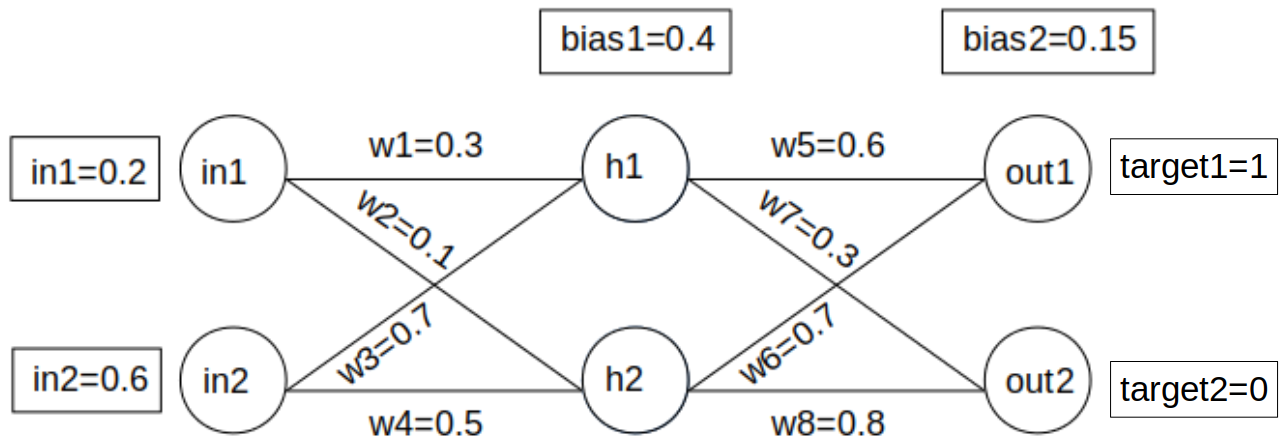
\includegraphics[scale=0.35, \keepaspectratio]{nn.png} 
	
	\caption{Simple neural network.}
	\label{fig:markers}
\end{figure}
%\bibliographystyle{alpha}
%\bibliography{sample}

\end{document}
